\section{Theory}
\label{sec:bootstrap-consensus}
\begin{figure*}[t]
	\centering
	\begin{subfigure}[b]{0.24\linewidth}
		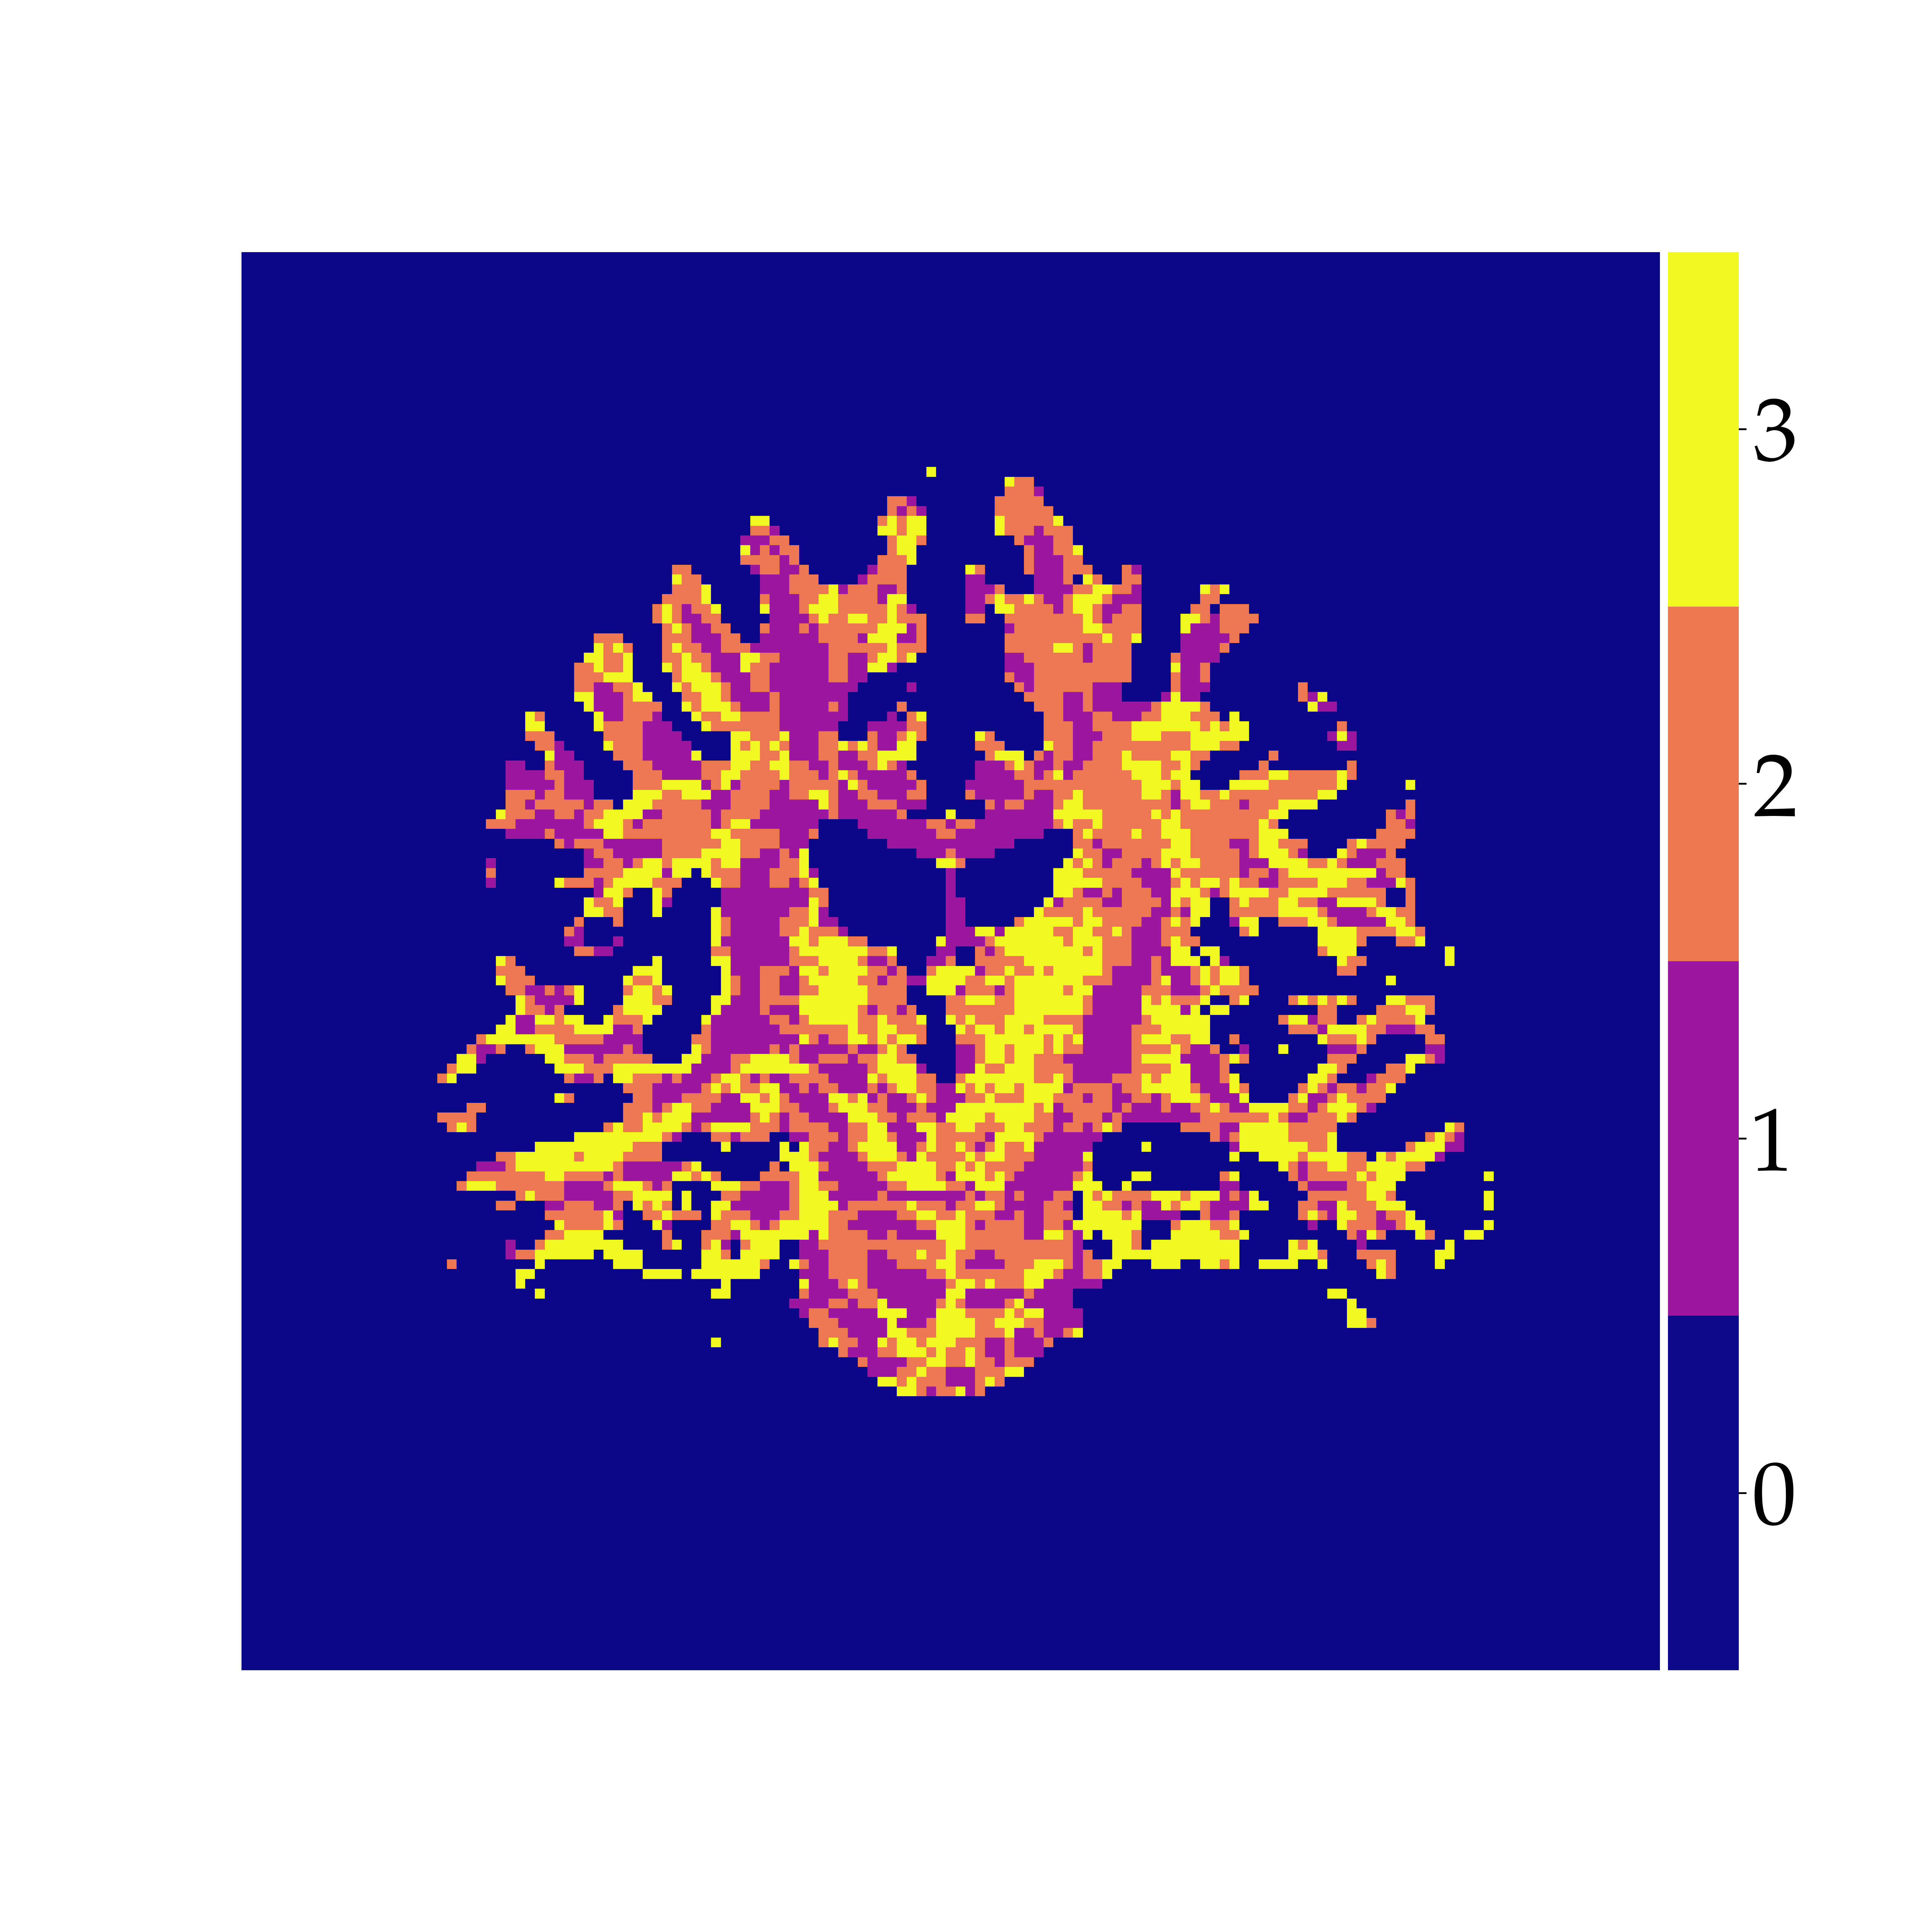
\includegraphics[width=\linewidth]{selected}
		\caption{The most likely number of fiber according to the
		selection model. {\color{white}asdfdsafdsfdsa}}
		\label{fig:selected-uncertainty:rank-original}
	\end{subfigure}
	\begin{subfigure}[b]{0.24\linewidth}
		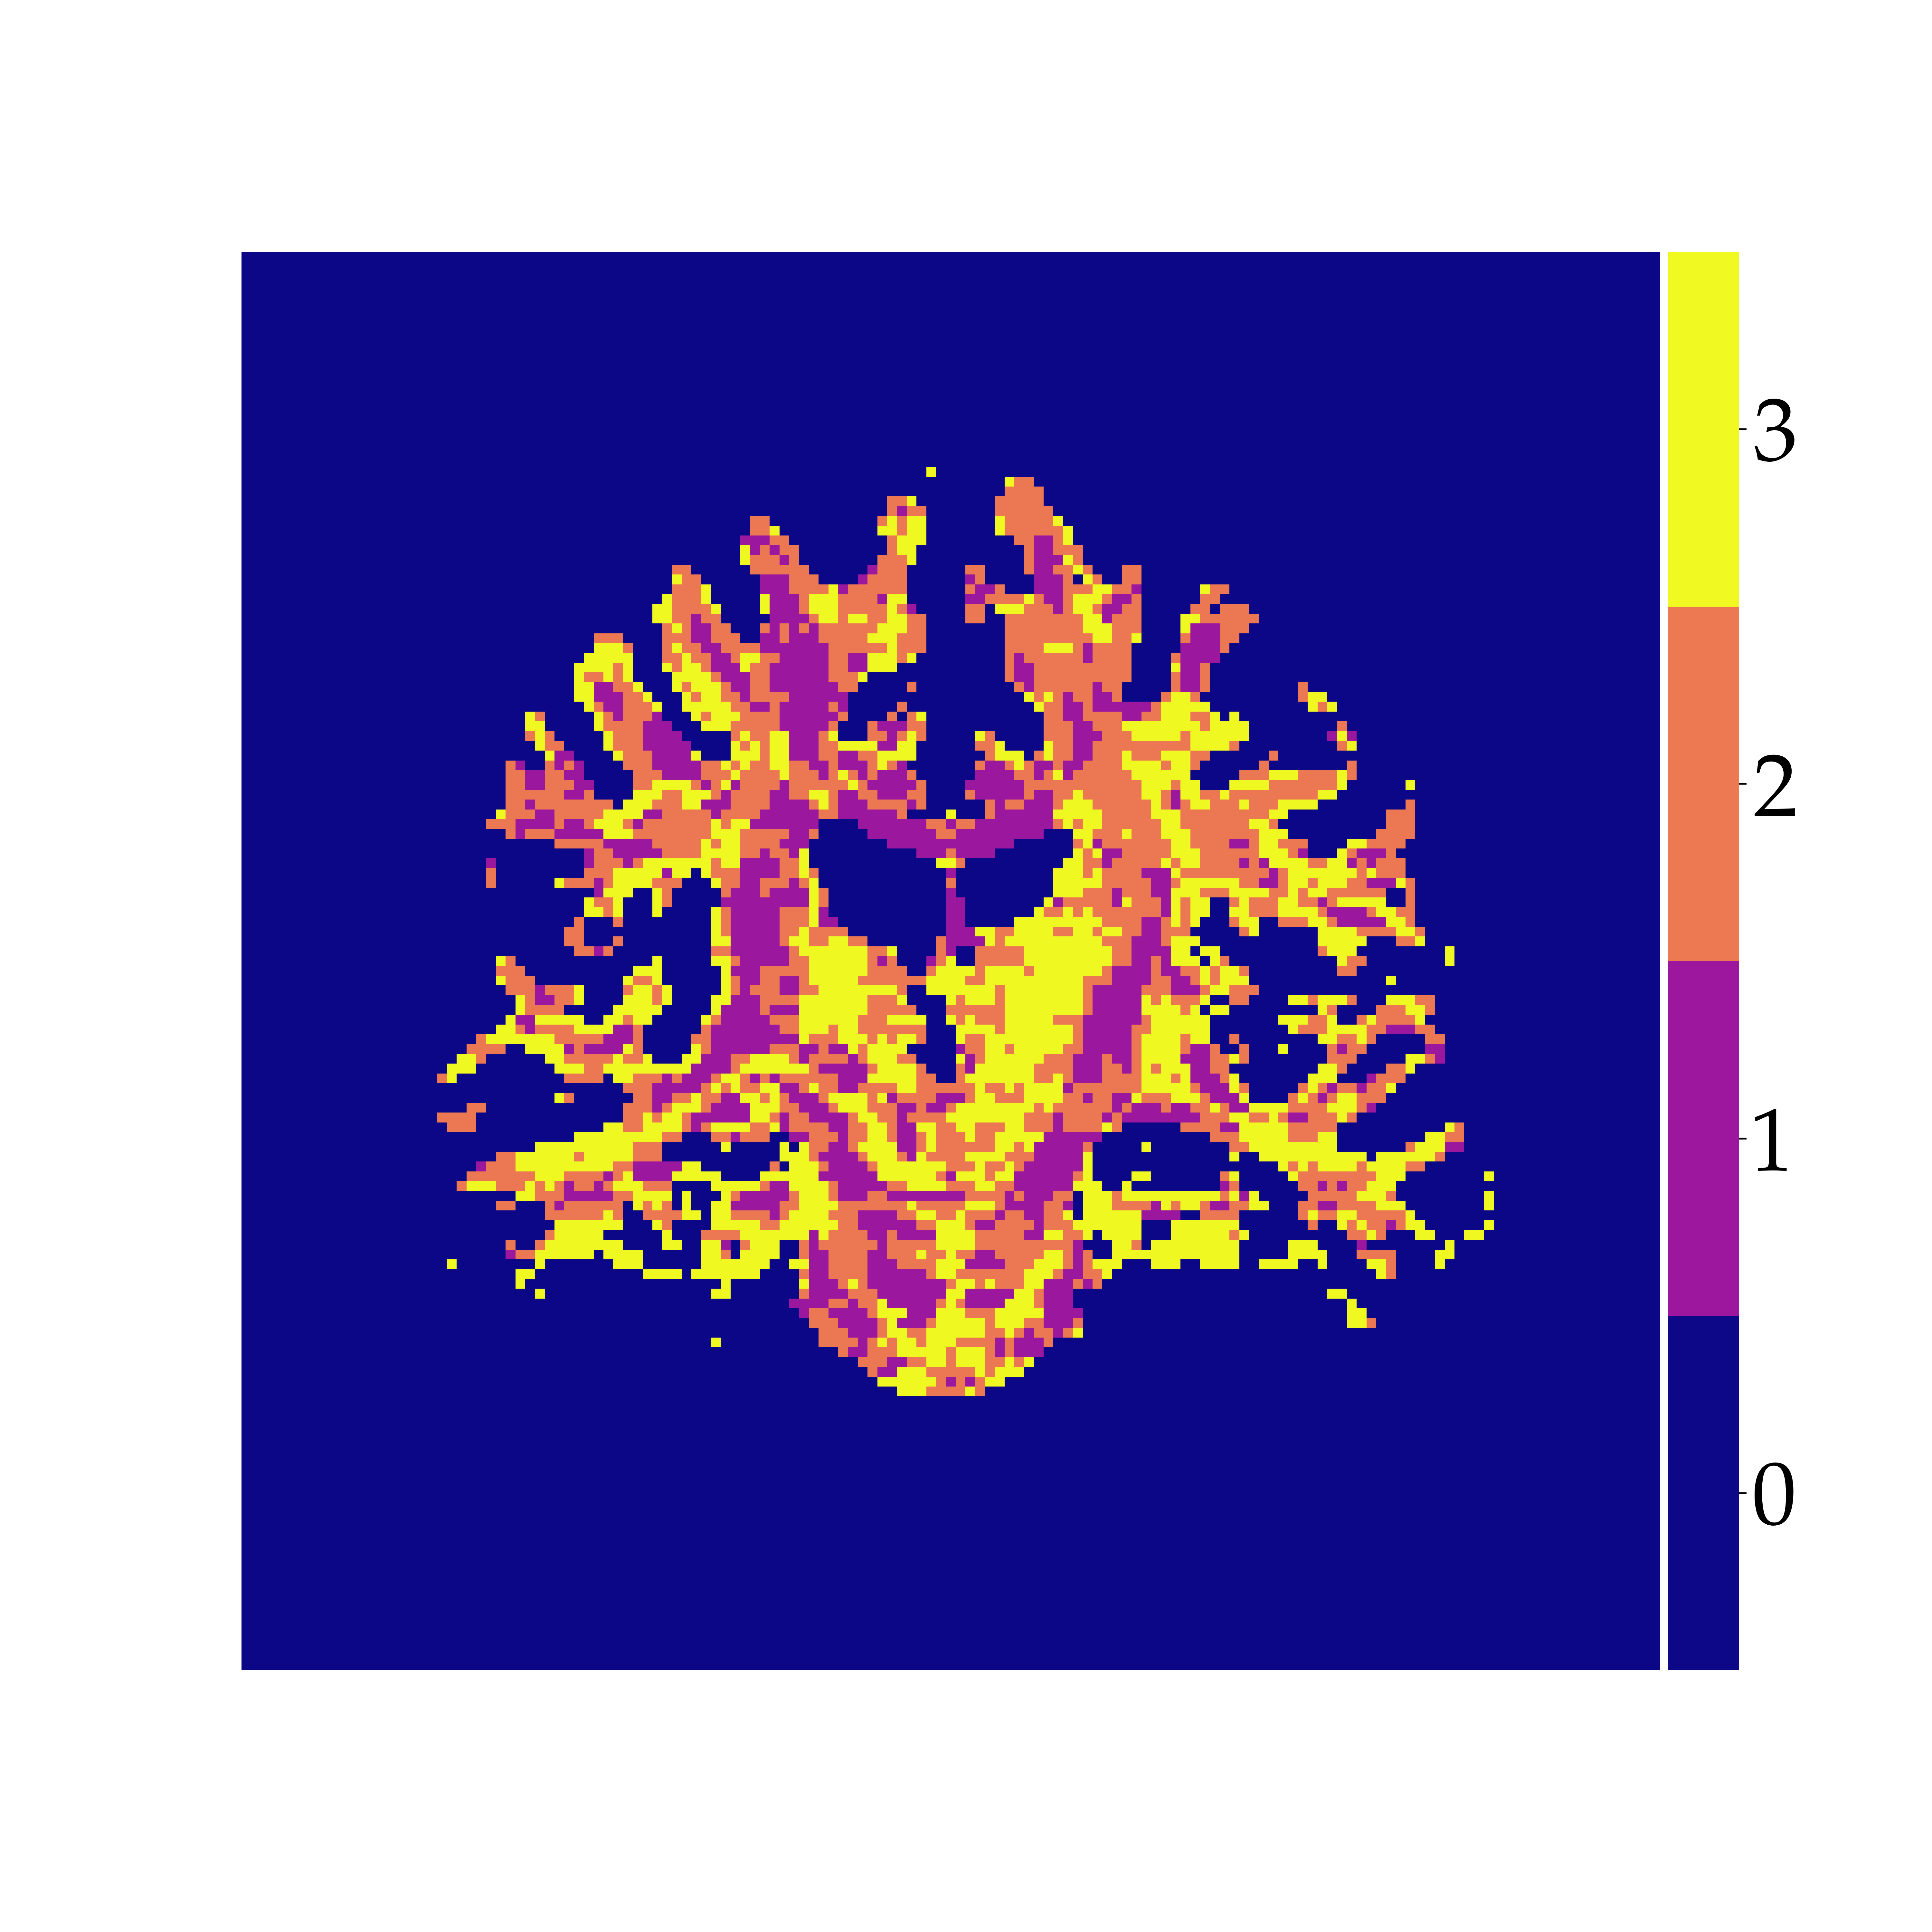
\includegraphics[width=\linewidth]{selected-bootstrap}
		\caption{The most like number of fibers over all
		bootstraps.{\color{white}iiiiiiiiiiii asdfdsafdsfdsa}}
		\label{fig:selected-uncertainty:rank}
\end{subfigure}  
	\begin{subfigure}[b]{0.24\linewidth}
		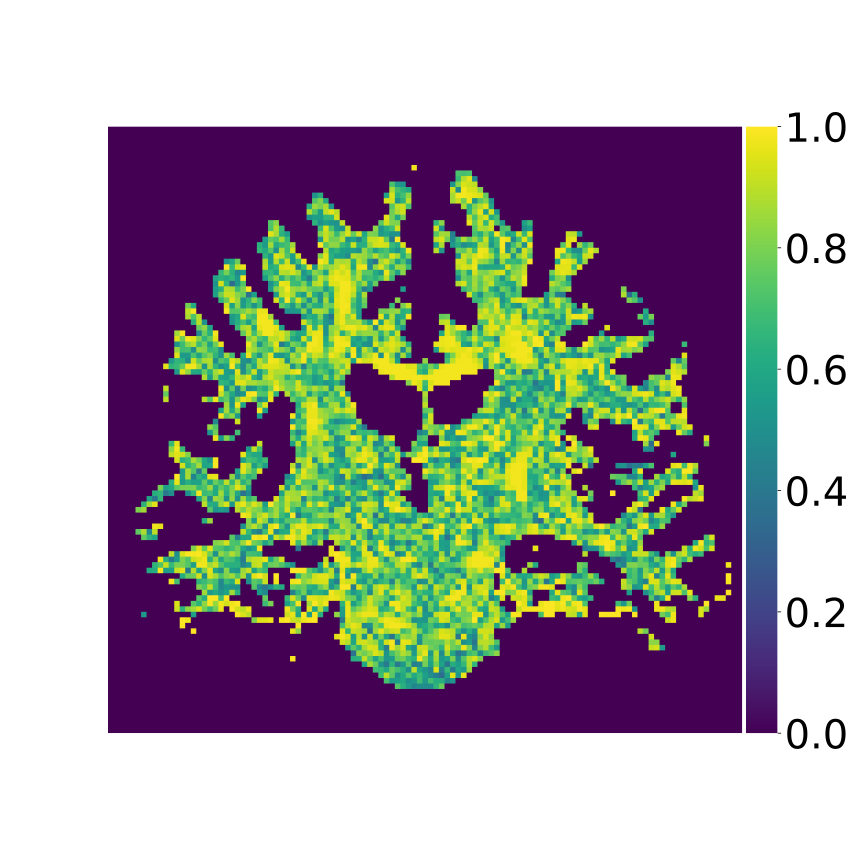
\includegraphics[width=\linewidth]{uncertainty}
		\caption{Certainty of the selected model.
		{\color{white}assdfsddfasd asdfdsafdsfdsa asdfsdafdfsfdfa}}
		
		\label{fig:selected-uncertainty:unc-original}
	\end{subfigure}
	\begin{subfigure}[b]{0.24\linewidth}
		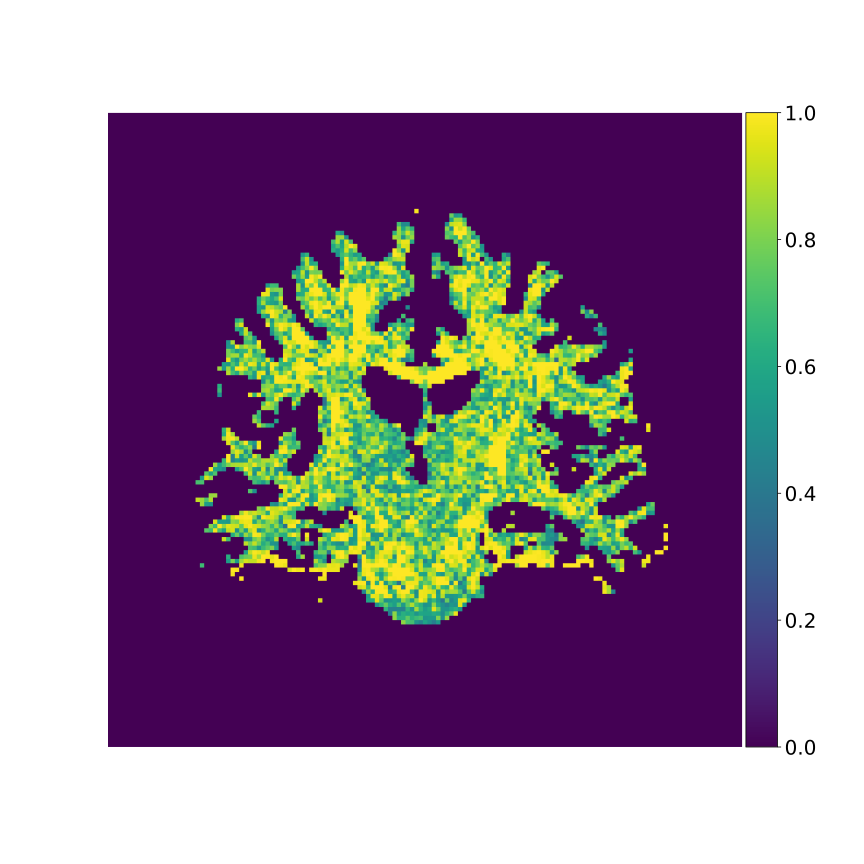
\includegraphics[width=\linewidth]{uncertainty-bootstrap}
		\caption{Number of bootstraps, which selected the most likely
		model over all bootstraps.}
		\label{fig:selected-uncertainty:unc}
	\end{subfigure}
	\caption{Comparison of model selection with and without bootstrapping.
	We denote that the Bayesian model is resistant against noise in the
sense that it selects in most cases the same model as the selection model
applied to the original data. However, it is also sensitive to noise, i.e. it
does not select always the same model.}
	\label{fig:selected-uncertainty}
\end{figure*}

Most bootstrap approaches in the context of dMRI are used  to generate
probabilistic tractographies out of deterministic tracking approaches. Such
approaches are reviewed in Section \ref{sec:related}. 

Our first novel contribution is to determine the uncertainty caused by
measurement errors to the proposed models in a systematical way. Therefore, wild bootstrapping is used to create
noisy resamples out of the measurements. The resampled data is then processed
and the parameters of a Watson distribution are evaluated to measure the
uncertainty which is propagated through the dMRI pipeline. 

As a second contribution we introduce a novel model, which reduces the measurement
uncertainty by incorporating all bootstraps into a new bootstrap consensus model.

\subsection{Wild Bootstrapping}
To evaluate the impact of measurement errors we use wild bootstrapping. It
has been shown in many cases that it is well suited within the context of dMRI and
is a straightforward way to
resample the original measurement without redoing the measurement process
\cite{Jones:2008}.

To create bootstrap samples the following process is applied. As a first step the model is fitted to the data. We obtain a fODF
$\hat{\mathcal{T}}$ and can calculate residual of Eq. (\ref{eq:sd-min}) 
\[ \hat{\varepsilon} = S - M\hat{\mathcal{T}} .\] 
A new bootstrap realization is calculated by 
\[ y^{*} = M\hat{\mathcal{T}}  + \hat{\varepsilon} v , \]
where $v$ denotes a random draw from the $n$ dimensional Rademacher distribution
\[ f \left( \mathbf{k} \right) \coloneqq  \begin{cases} \nicefrac{1}{2} \text{ if }
		\mathbf{k}_i=-1 \\
		\nicefrac{1}{2} \text{ if } \mathbf{k}_i=1 \\
		0 \text { otherwise } 
\end{cases} \text{ for } i \in \left\{ 1\dots n \right\} . \]
 Finally the model is fitted to the bootstrap realization. This process is repeated $m$
times to create a sample size of $m$ bootstraps.

For each sampled fODF we calculate the low-rank approximation of rank $3$
and with the obtained residuals also the selection and average model as it is
described in the previous section.

As a first contribution we investigate the distribution of the selected ranks
over all bootstrap. Therefore, we have simulated 100 bootstraps and applied the
selection model to all of them. The most
likely model in the original data is plotted in Fig.
\ref{fig:selected-uncertainty:rank-original} and the uncertainty of the selected model is
plotted in \ref{fig:selected-uncertainty:unc-original}. The generalization to the bootstrap model is
plotted right to the plots with the original data. Here the most likely number of fibers is
calculated by selecting the model, which occurs most in bootstraps. The count of
occurrences can be interpreted as uncertainty, e.g. if the selection model takes
always the same model not mattering the bootstrap errors, it is very certain
that this model fits the data well and vice versa.  
In most cases the selection model coincides with the most bootstraps. Only in
$14.1\%$ of the voxels withing the white matter area the selected rank differs
by $1$ and in $0.8\%$ the rank differs by $2$. Also regions which are quiet
certain are stay certain under bootstrapping. Therefore, we conclude that the
Bayesian posterior model is sensitive to noise and small changes in the data can
lead to different outcomes. 

\subsection{Bootstrap Consensus Model}
\begin{figure*}[t]
	\centering
	\begin{subfigure}[b]{0.33\linewidth}
		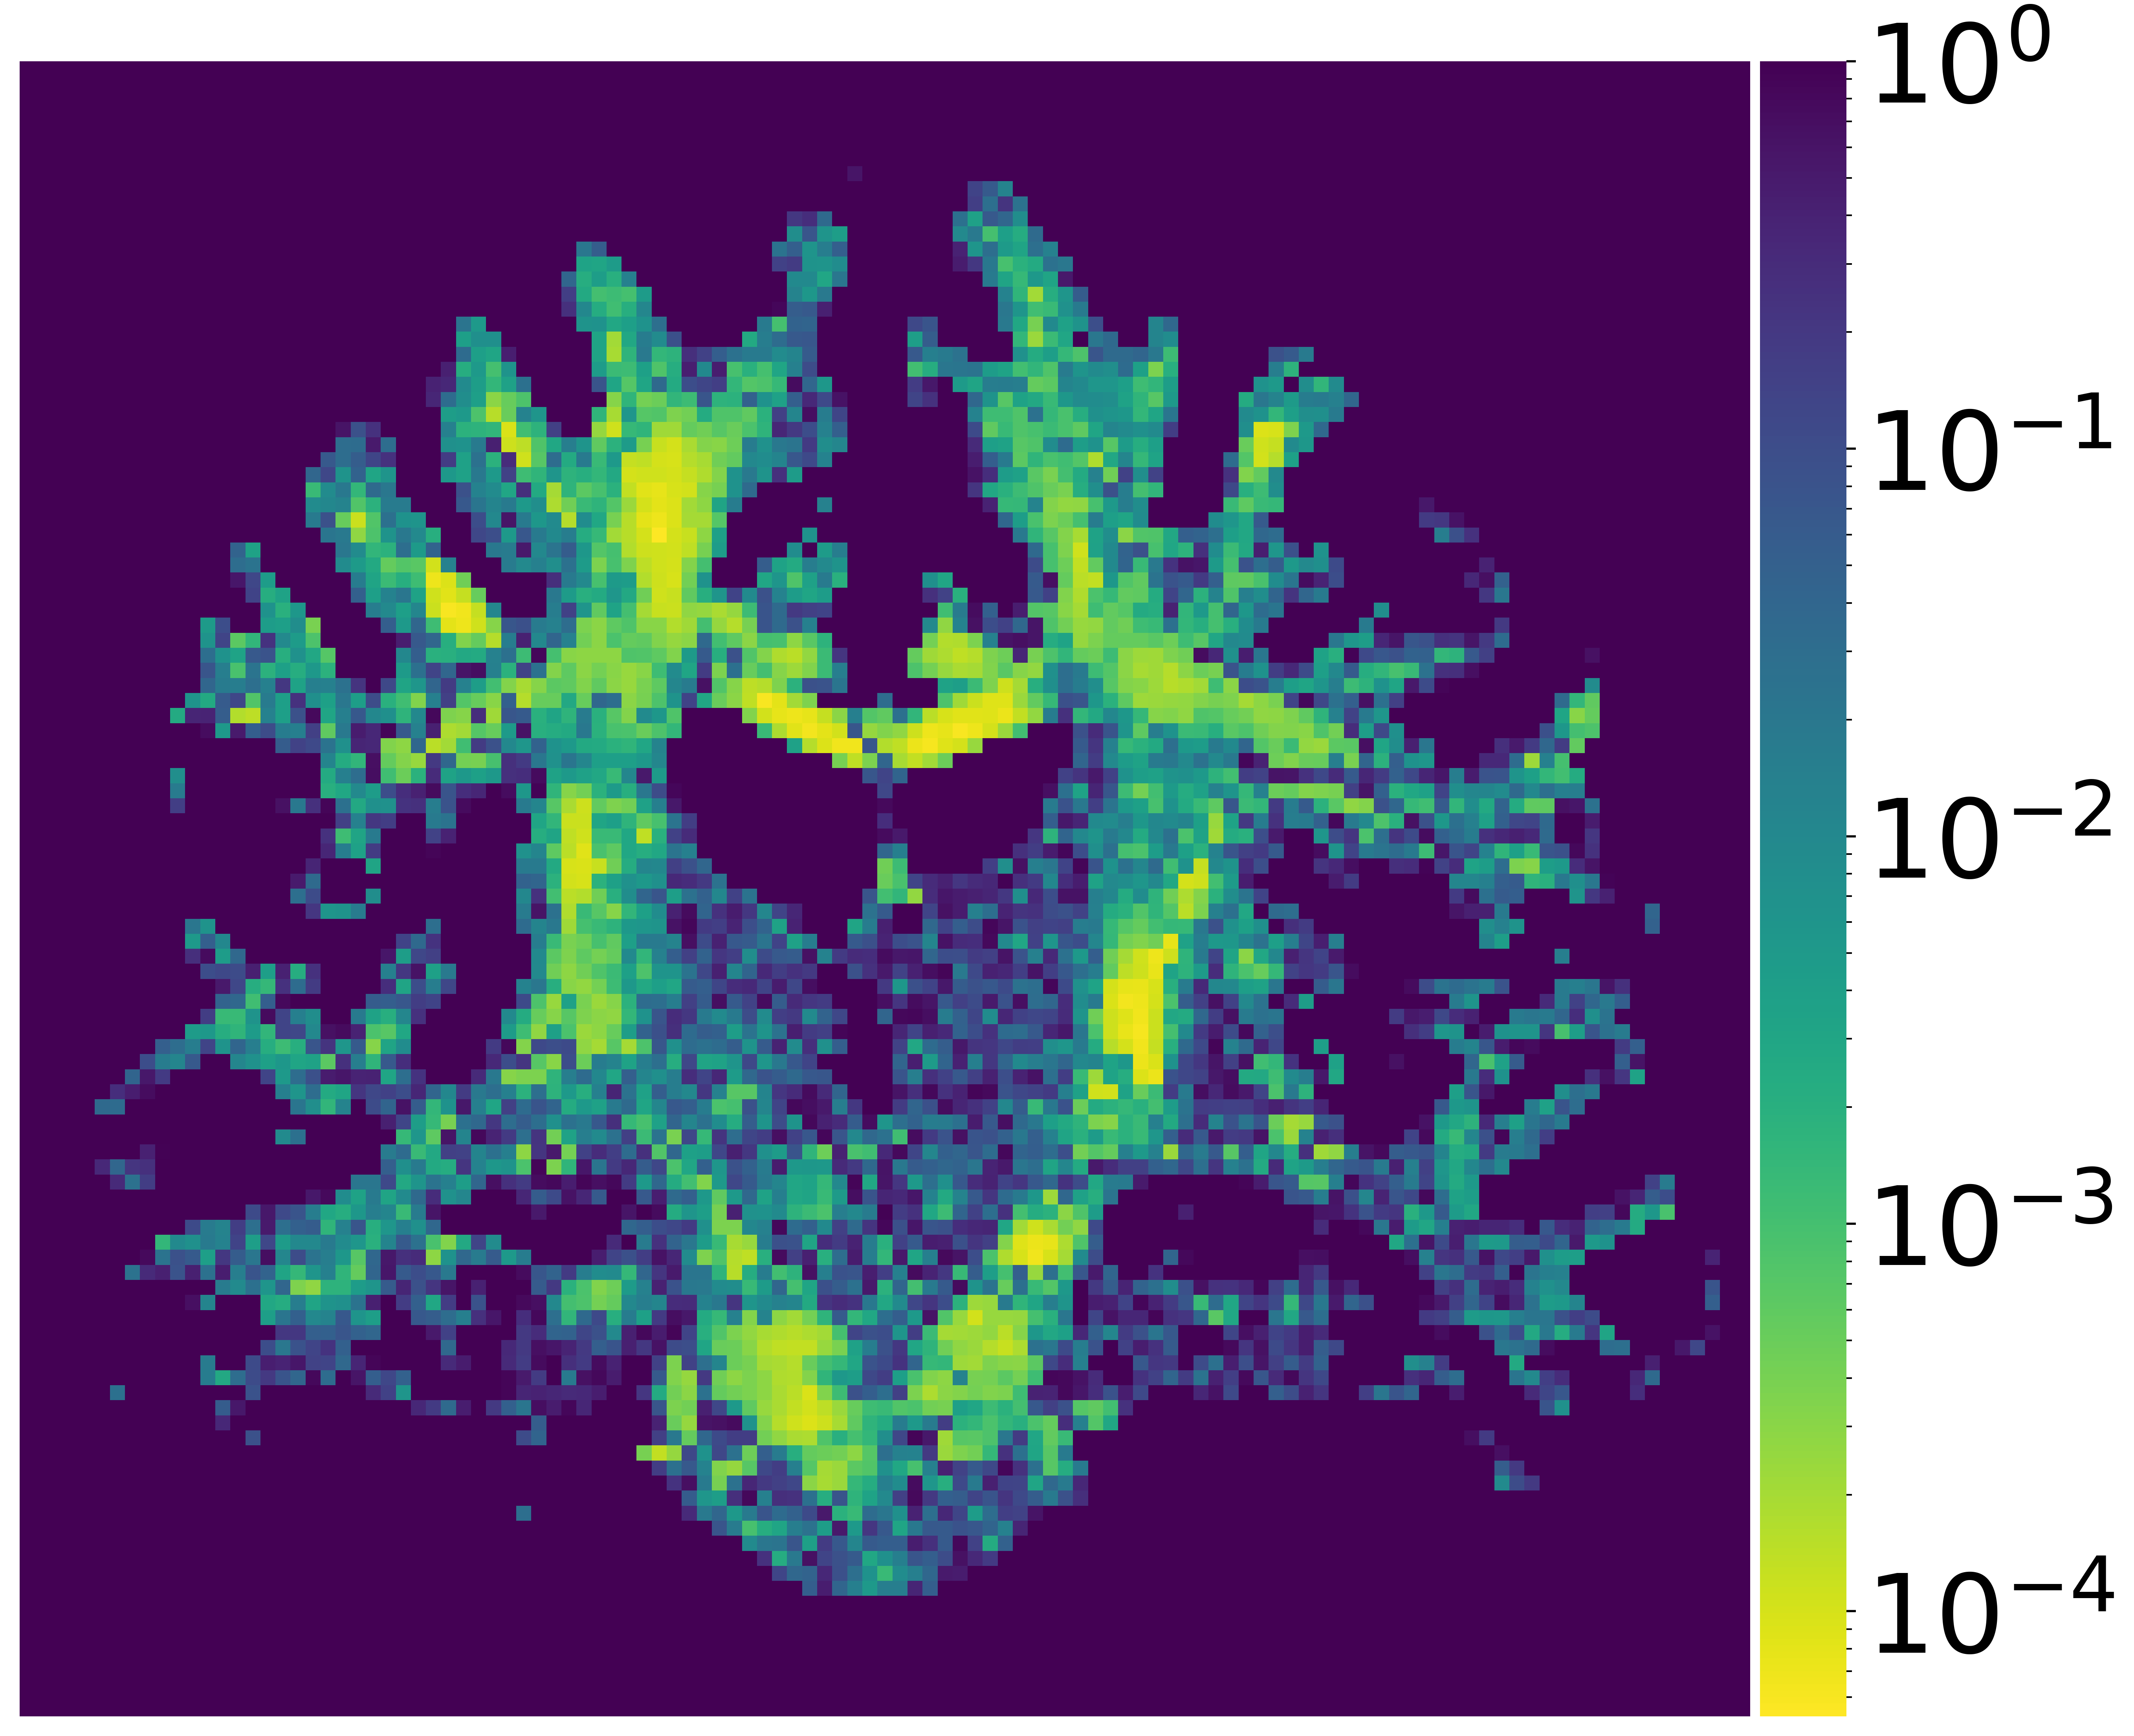
\includegraphics[width=\linewidth]{sel-bootstrap-maindir}
		\caption{Selection model}
		
	\end{subfigure}
	\begin{subfigure}[b]{0.33\linewidth}
		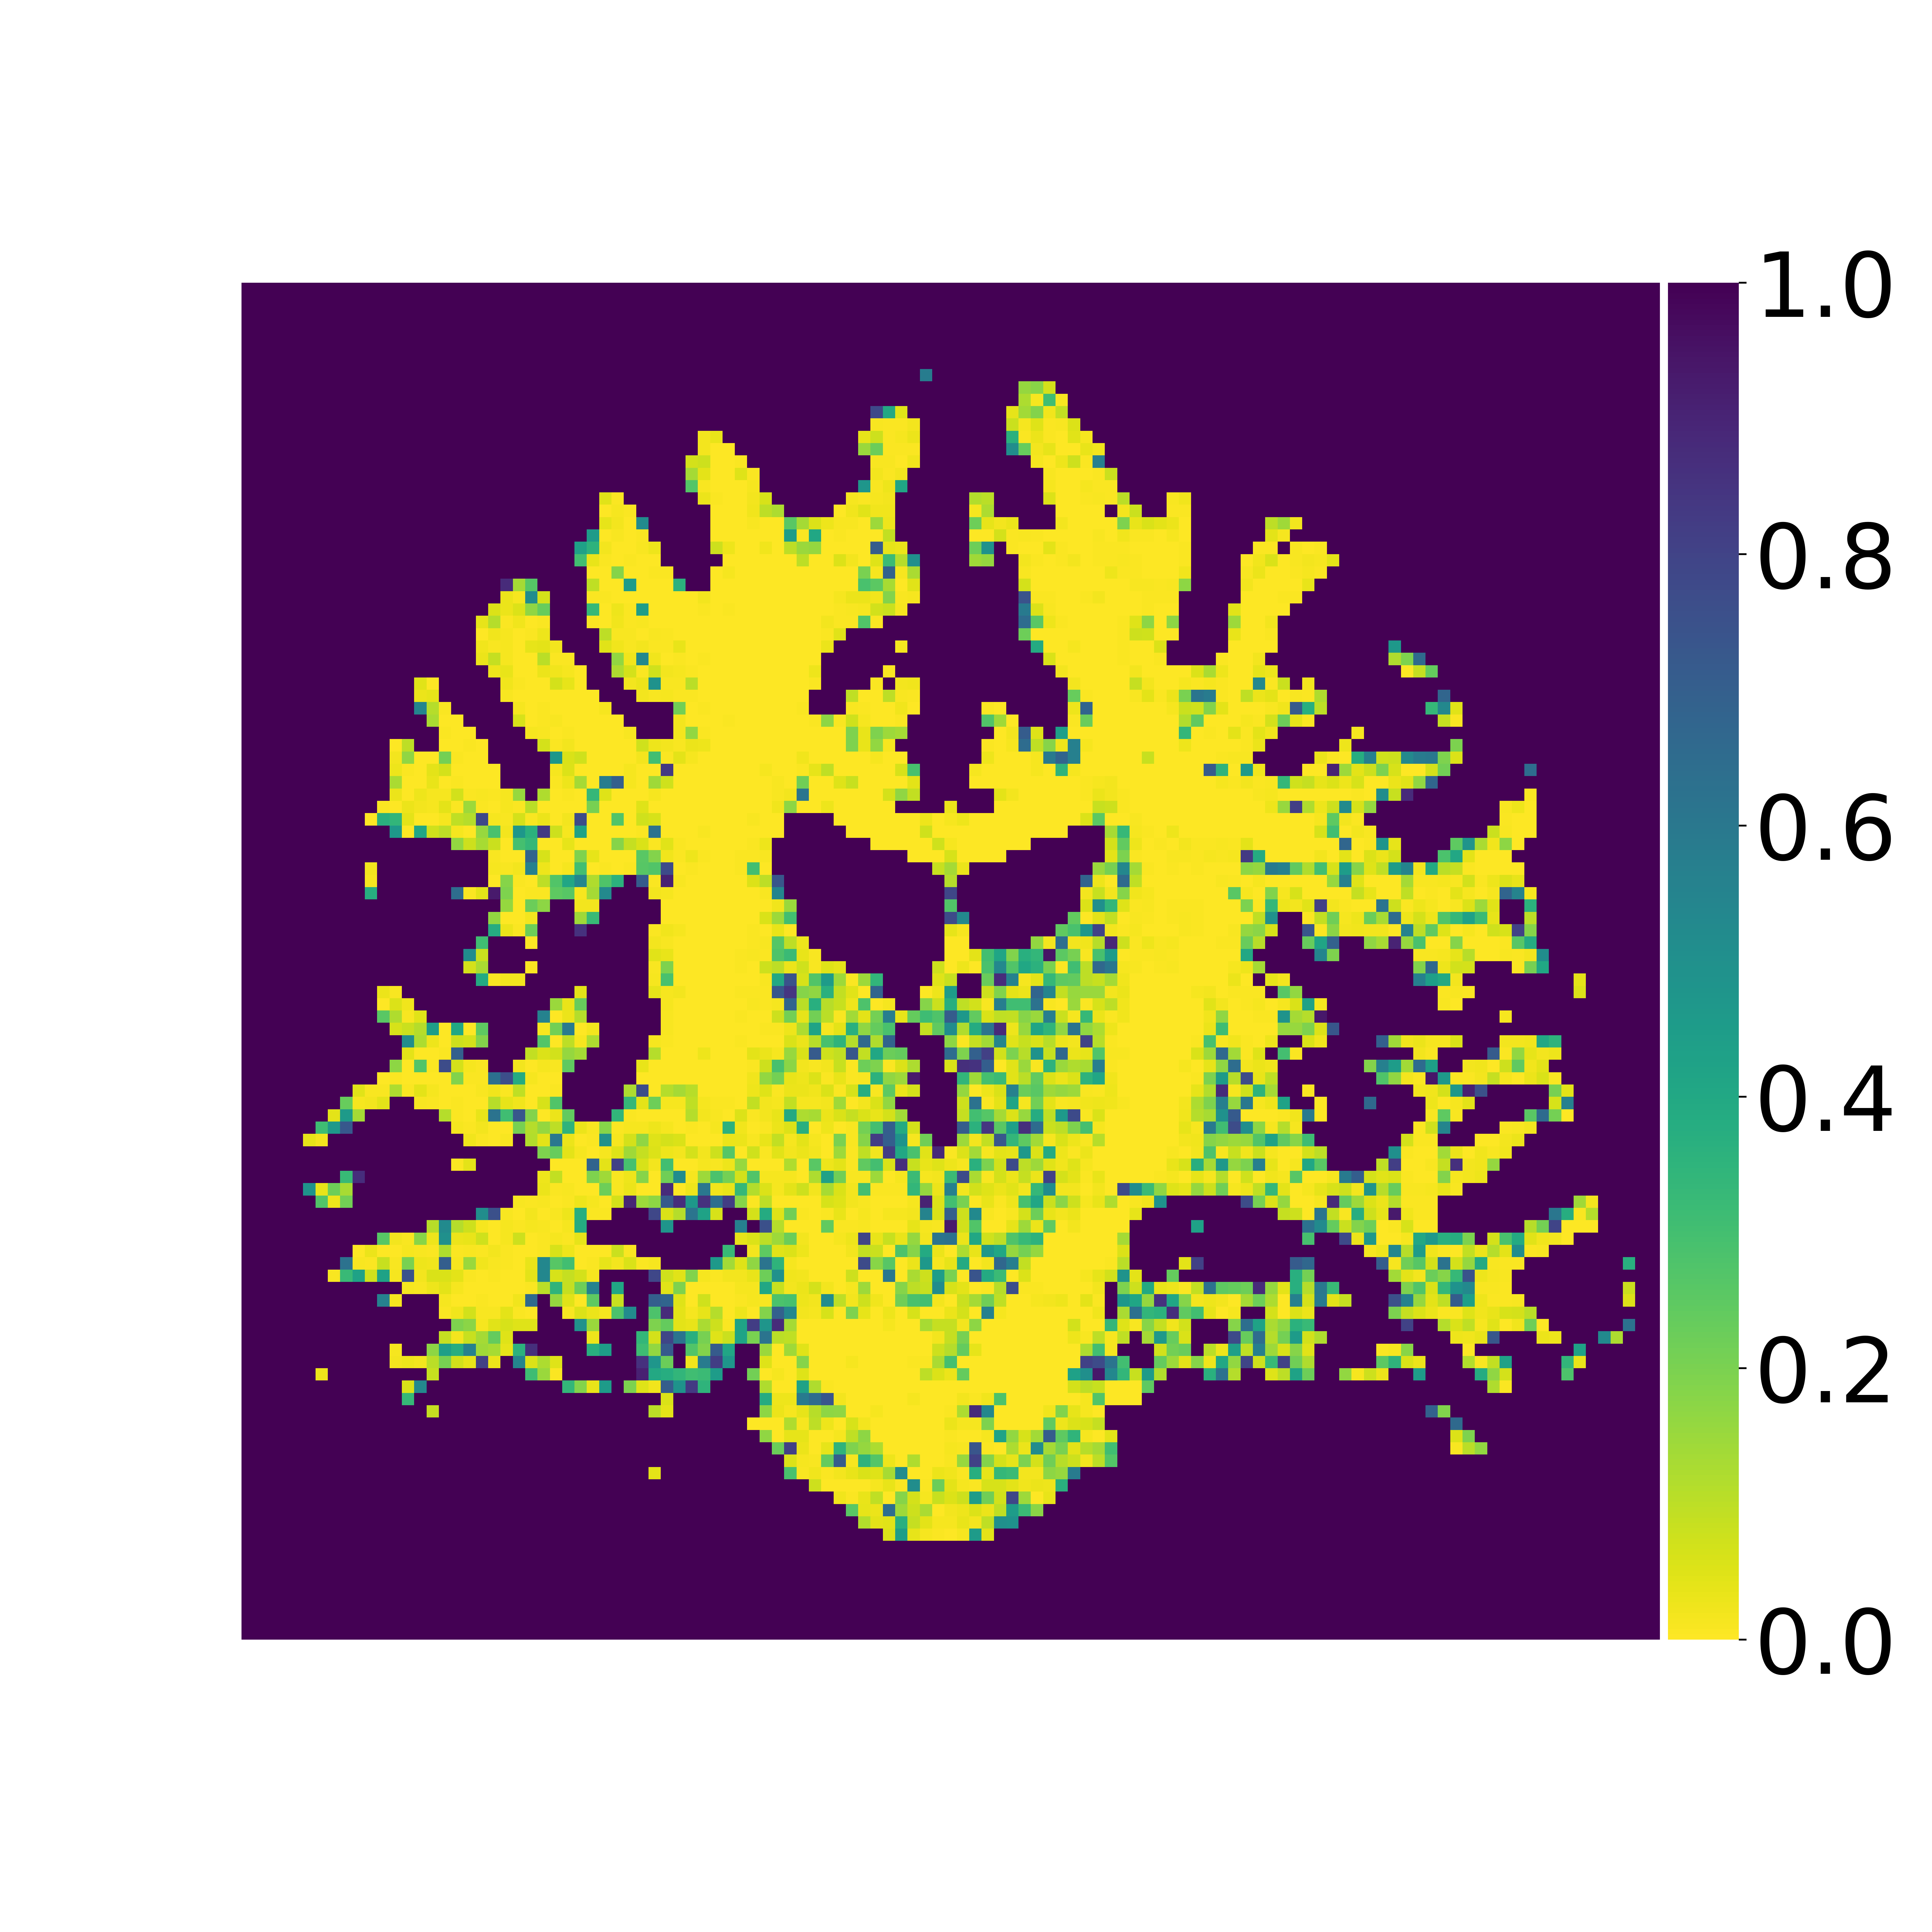
\includegraphics[width=\linewidth]{avg-bootstrap-maindir}
		\caption{Average model}
	\end{subfigure}
	\begin{subfigure}[b]{0.33\linewidth}
		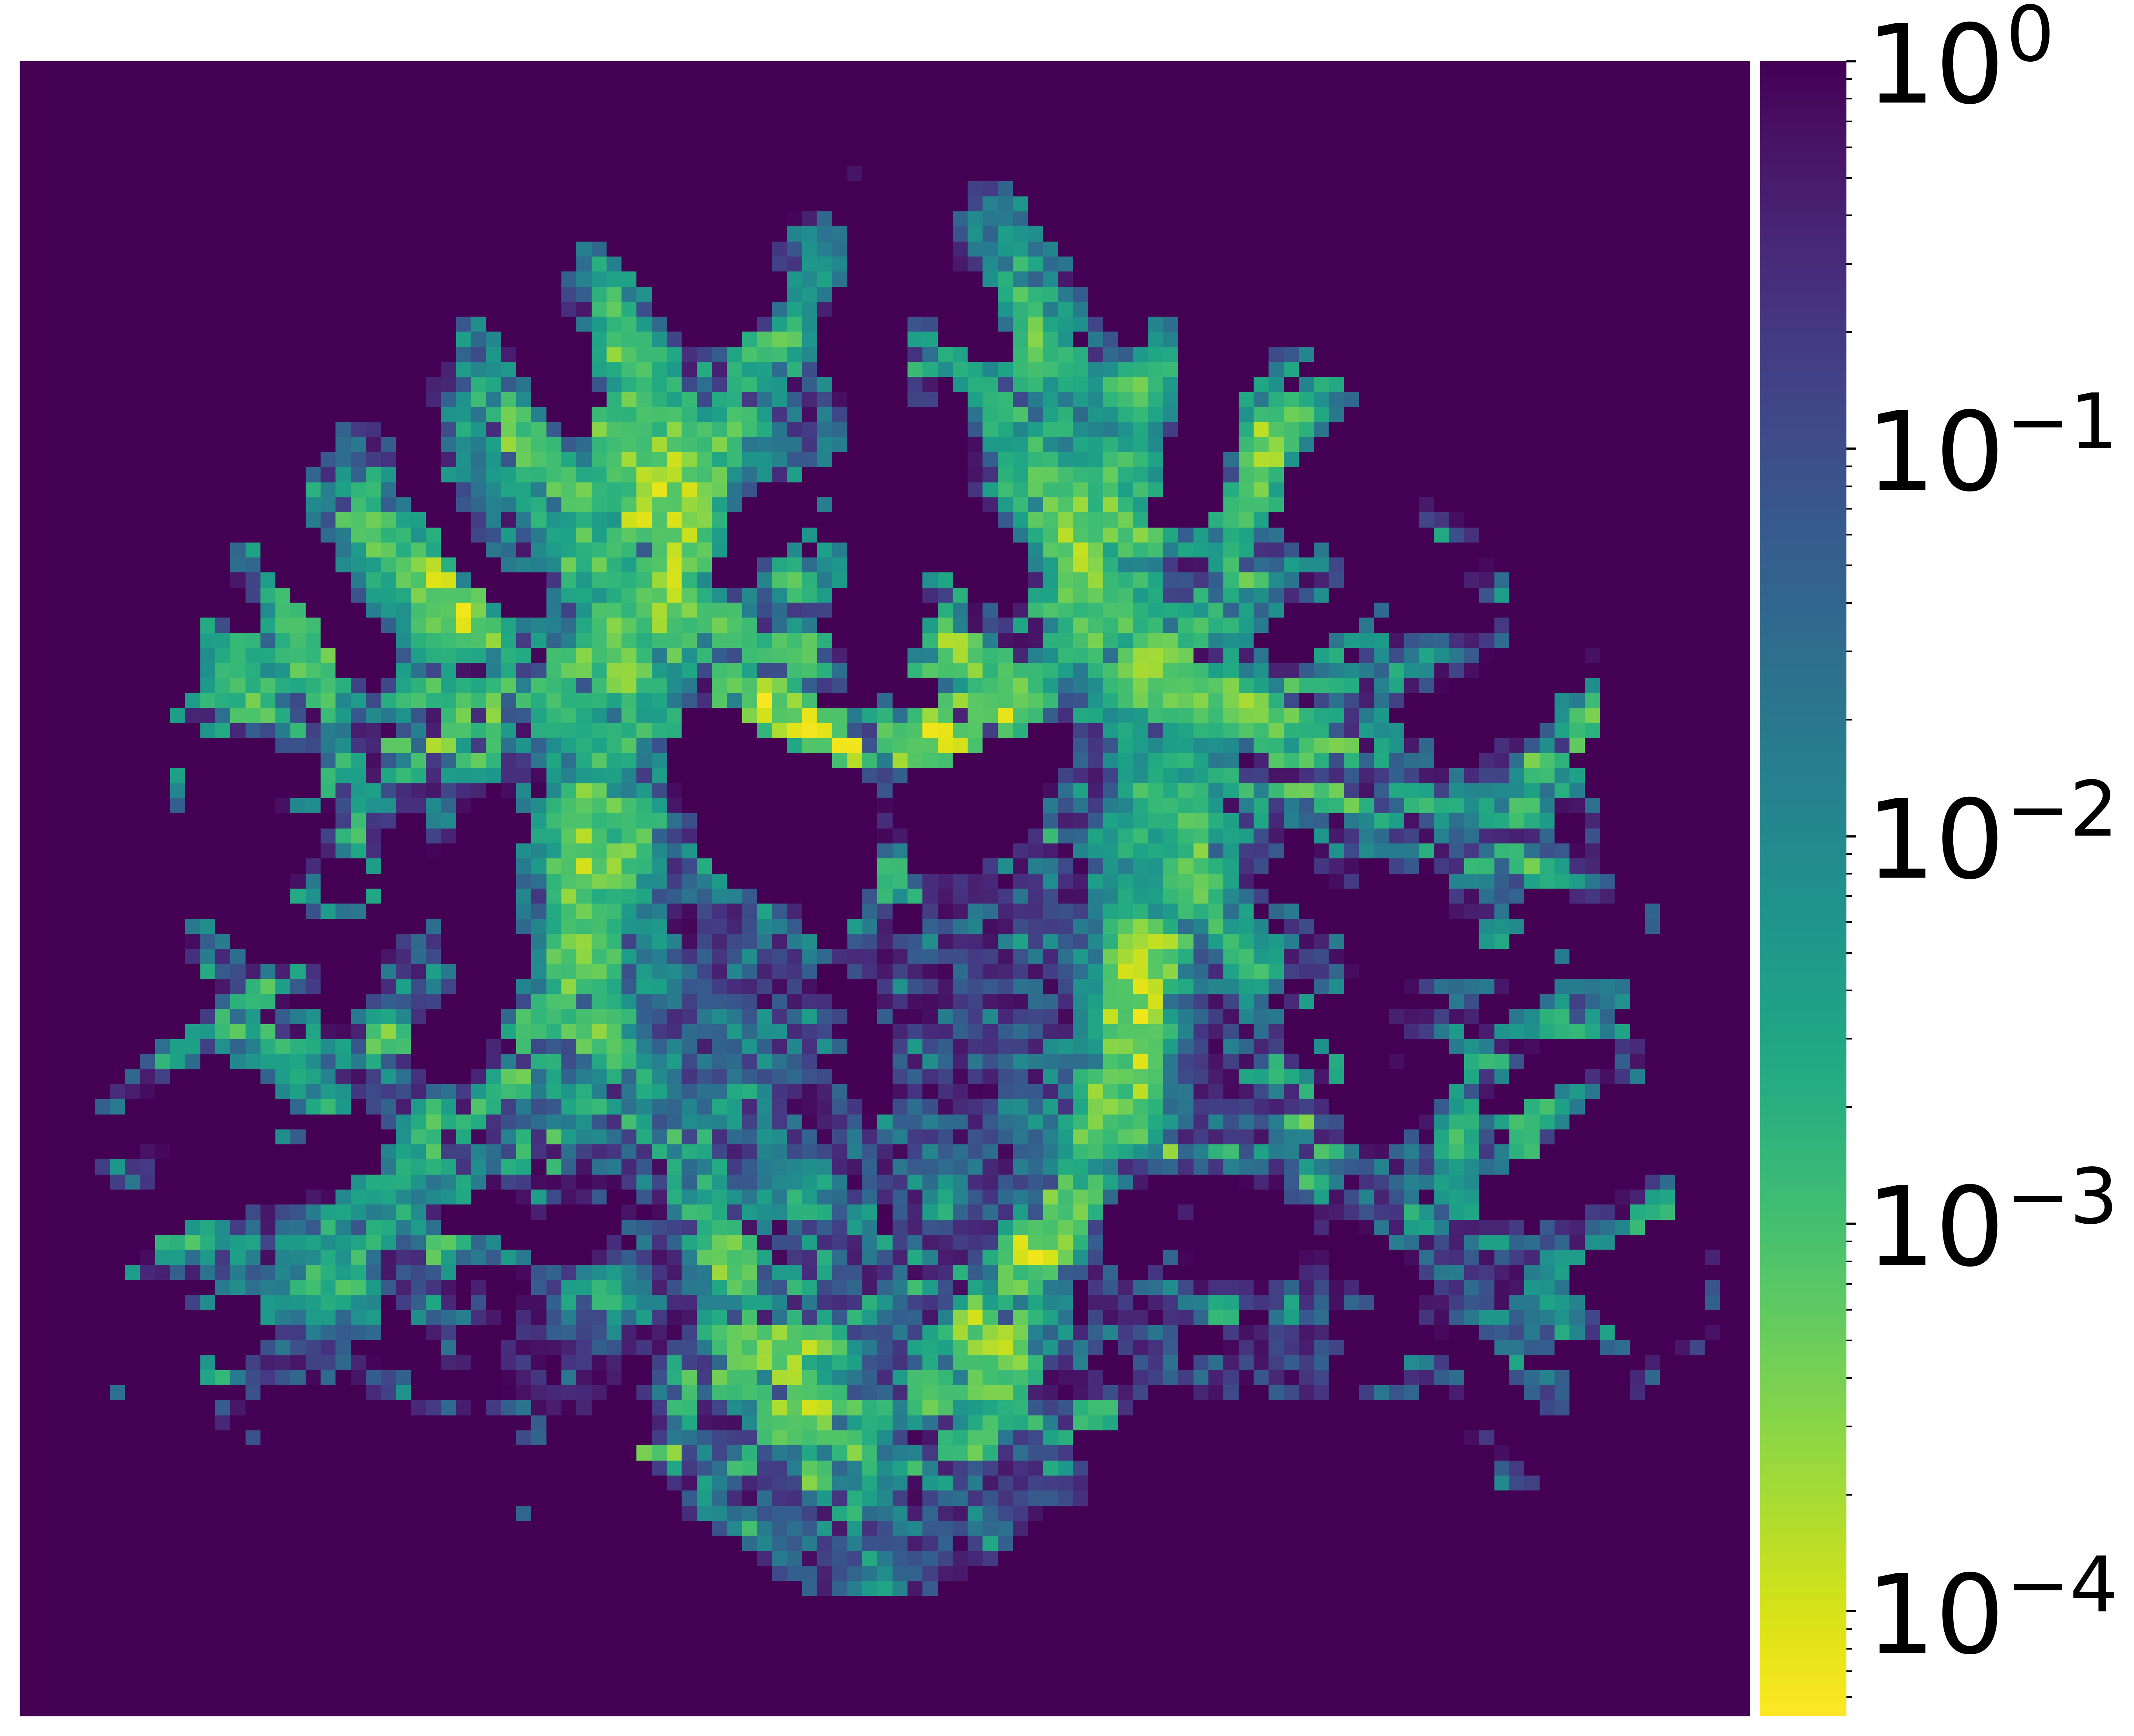
\includegraphics[width=\linewidth]{rank-bootstrap-maindir}
		\caption{Rank 3 model}
	\end{subfigure}

	\caption{Redefined orientation dispersion index calculated for the main
		direction (top row). The directions are ordered by volume fraction.
Within the main direction it is visible that the dispersion in the rank $3$
model is higher than in the both other models, which indicates a higher
susceptibility to noise. }
	\label{fig:dispersion}
\end{figure*}


Instead of using the bootstrap samples to produce a probability density map of
streamlines, we use it to reduce the measurement uncertainty by fusing the
information of all bootstraps into a new model. 
Therefore, the directions of all bootstraps get clustered to groups and the
group means are the new directions.

To build a consensus model we have to assign $n$ directions of $r$ bootstraps to $m$ groups on voxel
level where $m \geq n$. We initialize the process by setting the reference
direction for the $m$ groups as directions of
the low-rank $3$ model computed on the original data. Now each
direction of each bootstrap is assigned to a group such that the sum of
distances between group
reference and direction is minimized over all possible assignments to the
groups, i.e. we want to minimize the objective function 
\begin{align}
	T : \text{Sym} \left( n \right) & \mapsto \mathbb{R}_+ \nonumber \\
	Z & \rightarrow \sum \| \sgn \left( \langle \mathbf{v}_{Z\left( i
	\right)}, \bar{\mathbf{v}}_i \rangle \right) \mathbf{v}_{Z\left( i
	\right)} - \bar{\mathbf{v}}_i\| ,  
\end{align} 
where $\text{Sym}\left( n \right)$ denotes the symmetric group, 
$\bar{\mathbf{v}}_i$ denotes
the reference direction and $\mathbf{v}_i$ denotes the direction from the
bootstrap. To prevent wrong assignments if only one reference
direction is initialized we first assign the direction from the bootstrap with
the  highest fiber count to the
groups and update the uninitialized reference directions with the assignments.
Note that this does not necessary lead to a global optimum, but is in most cases
close to the optimum. 

To get deeper insights into the impact of the bootstrapping we fit a Watson
distribution to the grouped directions \cite{jupp_mardia_1999}. The Watson distribution is defined as  
\begin{align*}
	f : \mathbb{S}^2 & \longrightarrow  \mathbb{R}_+ \\
	\mathbf{x} & \longmapsto  M \left( \frac{1}{2}, \frac{3}{2} , \kappa
	\right)^{-1} \exp \left(  \kappa
	\left( \mathbf{\mu}^T \mathbf{x} \right)^2 
	\right) 	,  
\end{align*}
where $\kappa$ is the dispersion parameter, $\| \mathbf{\mu} \| = 1$ the
mean direction and $M$ be the confluent hypergeometric function. 

We use the Watson distribution because it has two main advantages. First of all, it is antipodal symmetric,
which fits our model assumption of indistinguishable $\pm \mathbf{v}$
directions. Secondly, it is one of the easiest models for axial data and
introduces the dispersion parameter, which gives  us deeper insights into the
uncertainty within the groups. 

In Fig. \ref{fig:dispersion} we have visualized the redefined orientation dispersion index
\cite{dispersionParameter}  
\[ OD = \frac{2}{\pi} \arctan \left( \frac{1}{\kappa} \right) \] 
for the selection, average and rank 3 model. This score is more intuitive since
it maps the low dispersion to low values and vice versa. 

It is visible that the
selection model and average model shows lower dispersion in large parts of the CC and CST tracts
compared to the rank $3$ model. This is caused by the
ability of the selection model to select the rank $1$ model in this areas, which
is not as susceptible to noise as higher rank models. I.e. the selection model
reduces the impact of measurement noise without explicitly being build for
this. The average model also benefits from the noise reduction, since the impact
of the lower rank models is high in these regions.
On the other hand the average model still contains more fiber directions, which
makes it more flexible compared to the selection model, which contains in many
voxels just a single fiber direction.
We conclude that average model fuses the stability from the selection model in
the mean direction and also the flexibility of the rank $3$ model, which can be
important in crossing regions.
Therefore, we assume that the impact to the average and rank $3$ model is lower
than to the selection model since we increase the flexibility by introducing
more directions into the consensus selection model. 



%%% Local Variables:
%%% mode: latex
%%% TeX-master: "../main"
%%% End:
